\documentclass[11pt]{article}
\usepackage[paperwidth=8.5in, paperheight=11in]{geometry}
\usepackage{algorithm}
\usepackage{algorithmicx}
\usepackage[noend]{algpseudocode}

\usepackage{../tjimo}

\newcommand{\sevenpoints}{Time limit: 45 minutes.}
\newcommand{\righthead}{\fdbox{Round}{Power}}

\usepackage{tikz}
\usepackage{amsmath}
\usepackage{amsthm}
\usepackage{amssymb}
%\usepackage{enumerate}
\usepackage{enumitem}
\usepackage{gensymb}
\usepackage{multicol}

%\begin{comment}
\def \answer{\comment}
\def \solution{\comment}
%\end{comment}

\begin{document}

\section{Introduction}

Unlike the other rounds, just getting the answer right is not enough on the Power Round. Make sure you explain your answer and use words to describe how you arrived at your answer. In the words of middle school math teachers across the nation -- no work, no credit!

\phantom{hi} \noindent This Power Round (worth 150 points) is divided into two sections. In the first section,  we will be proving shoelace for triangles. Finally, we will be proving the shoelace theorem in general in the third section.

\phantom{hi} \noindent Feel free to use results from previous problems on this round to prove a later problem (that is, you can use Problem 2 to prove Problem 3, but not vice versa). You do not need to have solved the earlier problem to cite its result.

\phantom{hi} \noindent Do not be afraid if this power round is difficult, we will grade leniently. However, this does not mean that you should not do your best - show all work!

\section{Recap}

The shoelace theorem can be used to calculate the area of polygons, given the Cartesian coordinates of the vertices. 

\begin{theorem}[The Shoelace Theorem] Suppose the polygon $P$ has vertices $(a_1, b_1)$, $(a_2, b_2)$, ... , $(a_n, b_n)$, listed in counterclockwise order. Then the area of $P$ is

\[\dfrac{1}{2} |(a_1b_2 + a_2b_3 + \cdots + a_nb_1) - (b_1a_2 + b_2a_3 + \cdots + b_na_1)|\]
\end{theorem}
\begin{comment}
The Shoelace Theorem gets its name because if one lists the coordinates in a column, 
\begin{align*} 
(a_1 &, b_1) \\ 
(a_2 &, b_2) \\ 
& \vdots \\ 
(a_n &, b_n) \\ 
(a_1 &, b_1) \\ 
\end{align*} 
and marks the pairs of coordinates to be multiplied, the resulting image looks like laced-up shoes.
\end{comment}

\begin{definition}
\[\left|\begin{array}{c c}a_1  & b_1 \\ a_2 &  b_2 \\ \vdots & \vdots \\ a_n & b_n \\ a_1 & b_1 \\ \end{array}\right| = \dfrac{1}{2} |(a_1b_2 + a_2b_3 + \cdots + a_nb_1) - (b_1a_2 + b_2a_3 + \cdots + b_na_1)|\]
Note that the shoelace theorem gets its name from the criss-crossing that results (in the first expression) when one marks the pairs of coordinates to be multiplied.
\end{definition}

\subsection{List of Facts}
Here are facts you may use from the practice power on this power round:

\begin{theorem}
The shoelace theorem applies if a triangle is entirely contained within the first quadrant and has a vertex located at the origin.
\end{theorem}

\begin{theorem}
The shoelace theorem is consistent when a triangle is rotated by $90\degree$ counterclockwise about the origin. 
\end{theorem}

\section{General Triangles}

\begin{problem}[5 points total]  Prove that the shoelace theorem is consistent with translation, or in other words, the triangle with vertices $(x_1, y_1), (x_2, y_2), (x_3, y_3)$ has the same area as the triangle with vertices $(x_1 - a, y_1 - b), (x_2 - a, y_2 - b ), (x_3 - a, y_3 - b)$. \end{problem}

\begin{solution}
Using shoelace on the triangle with vertices $(x_1, y_1), (x_2, y_2), (x_3, y_3)$ yields $\frac{1}{2}|x_1y_2+x_2y_3+x_3y_1-y_1x_2-y_2x_3-y_3x_1|$. Using shoelace on the triangle with vertices $(x_1 - a, y_1 - b), (x_2 - a, y_2 - b ), (x_3 - a, y_3 - b)$ yields \[\frac{1}{2}|(x_1-a)(y_2-b)+(x_2-a)(y_3-b)+(x_3-a)(y_1-b)-(y_1-b)(x_2-a)-(y_2-b)(x_3-a)-(y_3-b)(x_1-a)|\]
\[=\frac{1}{2}|x_1y_2-bx_1-ay_2+ab+x_2y_3-bx_2-ay_3+ab+x_3y_1-bx_3-ay_1+ab \]
\[-y_1x_2+ay_1+bx_2-ab-y_2x_3+ay_2+bx_3-ab-y_3x_1+ay_3+bx_1-ab|\]
\[=\frac{1}{2}|x_1y_2+x_2y_3+x_3y_1-y_1x_2-y_2x_3-y_3x_1|\]
Thus, we are done.
\end{solution}

\begin{problem}[10 points total]  Prove that the shoelace theorem applies for all triangles. \end{problem}

\begin{solution}
We begin by translating each triangle so that one vertex lies at the origin and the rest of it lies entirely in one quadrant. This is possible since if we draw a box around the triangle, one of the vertices of the box will always line up with that of the triangle. Afterwards, we can rotate the triangle $90 \degree$ about the origin until it lies entirely in the first quadrant. Since the shoelace theorem applies in this case and is consistent with every transformation, the shoelace theorem applies for all triangles.
\end{solution}

\subsection{Clockwise or Counterclockwise?}
Note that for the 6 ways of ordering the vertices of the triangle, each ordering will traverse the vertices in either a clockwise or a counterclockwise direction. 
\newline \noindent Let the three vertices of triangle $ABC$ lie at $(x_1, y_1), (x_2, y_2),$  and $(x_3, y_3)$, in counterclockwise direction starting at $(x_1, y_1)$. 

\begin{problem}[5 points total]  Prove that
\[\left|\begin{array}{c c} x_1 &  y_1 \\ x_2  & y_2 \\ x_3  & y_3 \\ x_1 & y_1 \\ \end{array}\right| = 
\left|\begin{array}{c c} x_2  & y_2 \\ x_3  & y_3 \\ x_1 &  y_1 \\ x_2 & y_2 \\ \end{array}\right| = 
\left|\begin{array}{c c} x_3  & y_3 \\ x_1 &  y_1 \\ x_2  & y_2 \\ x_3 & y_3 \\ \end{array}\right| = 
-\left|\begin{array}{c c}x_1 &  y_1 \\ x_3  & y_3 \\ x_2  & y_2 \\ x_1 & y_1 \\ \end{array}\right| = 
-\left|\begin{array}{c c} x_2  & y_2 \\ x_1  & y_1 \\ x_3 &  y_3 \\ x_2 & y_2 \\ \end{array}\right| = 
-\left|\begin{array}{c c} x_3  & y_3 \\ x_2 &  y_2 \\ x_1  & y_1 \\ x_3 & y_3 \\ \end{array}\right|\]
\end{problem}

\begin{solution}
Let $S_1$ be the sum $x_1y_2 + x_2y_3 + x_3y_1$, and $S_2$ be the sum $x_2y_1 + x_3y_2 + x_1y_3$.
Note that the first three expressions are all equal to $S_1-S_2$ and the last three expressions are equal to $-(S_2-S_1) = S_1-S_2$. Thus, all six expressions are equal.
\end{solution}
\begin{problem}[10 points total]
Prove that if the vertices are listed counter-clockwise, the resulting expression is always positive. (Hint: transform each triangle so that it matches the case in problem on the practice power problem 4.)
\end{problem}

\begin{solution}
We begin by translating each triangle so that one vertex lies at the origin and the rest of it lies entirely in one quadrant. This is possible since if we draw a box around the triangle, one of the vertices of the box will always line up with that of the triangle. Afterwards, we can rotate the triangle $90 \degree$ about the origin until it lies entirely in the first quadrant. Note that this is doable because the shoelace theorem is consistent for all of the applied transformations. Also, rotation and translation do not change which way is counterclockwise. We have three cases:
\phantom{blahbity blah} 
\begin{multicols}{3}
\begin{enumerate}
\item $x_1 \leq x_2$ and $y_1 \geq y_2$
    \newline
    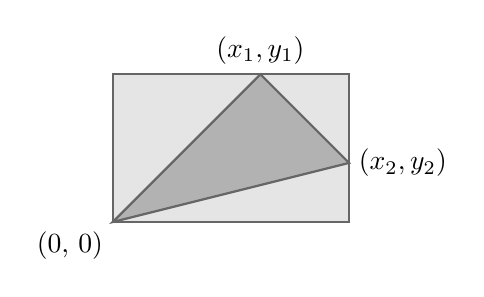
\begin{tikzpicture}
        \filldraw[color = black!60, fill = black!10, thick] (0, 0) -- (3, 0) -- (3, 1.875) -- (0, 1.875) -- cycle;
        \filldraw[color = black!60, fill = black!30, thick] (0, 0) -- (3, .75) -- (1.875, 1.875) -- cycle;
        \node at (0, 0) [below left] {(0, 0)};
        \node at (3, .75) [right] {$(x_2, y_2)$};
        \node at (1.875, 1.875) [above] {$(x_1, y_1)$};
    \end{tikzpicture}
\item $x_1 > x_2$, $y_1 > y_2, \frac{y_2}{x_2} < \frac{y_1}{x_1}$
    \newline
    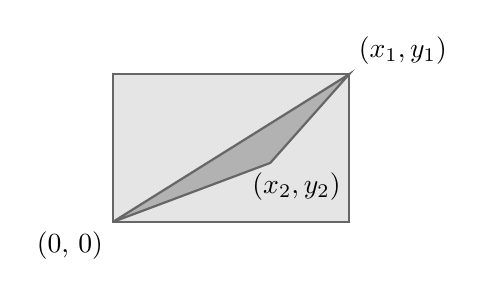
\begin{tikzpicture}
        \filldraw[color = black!60, fill = black!10, thick] (0, 0) -- (3, 0) -- (3, 1.875) -- (0, 1.875) -- cycle;
        \filldraw[color = black!60, fill = black!30, thick] (0, 0) -- (3, 1.875) -- (2, .75) -- cycle;
        \node at (0, 0) [below left] {(0, 0)};
        \node at (3, 1.875) [above right] {$(x_1, y_1)$};
        \node at (1.65, .75) [below right] {$(x_2, y_2)$};
    \end{tikzpicture}
\item $x_2 > x_1$, $y_2 > y_1, \frac{y_2}{x_2} < \frac{y_1}{x_1}$
    \newline
    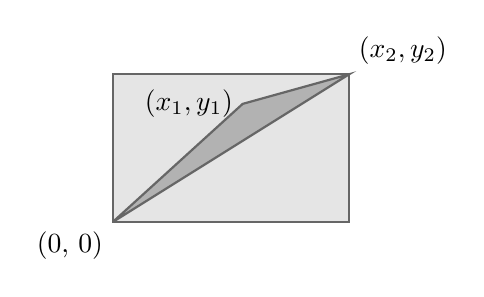
\begin{tikzpicture}
        \filldraw[color = black!60, fill = black!10, thick] (0, 0) -- (3, 0) -- (3, 1.875) -- (0, 1.875) -- cycle;
        \filldraw[color = black!60, fill = black!30, thick] (0, 0) -- (3, 1.875) -- (1.65, 1.5) -- cycle;
        \node at (0, 0) [below left] {(0, 0)};
        \node at (3, 1.875) [above right] {$(x_2, y_2)$};
        \node at (1.65, 1.5) [left] {$(x_1, y_1)$};
    \end{tikzpicture}
\end{enumerate}

\end{multicols}
In all cases, we are seeking to prove that $(0)(y_2) + (x_2)(y_1) + (x_1)(0) - (0)(x_2) - (y_2)(x_1) - (y_1)(0) > 0$, or $x_2y_1-y_2x_1 > 0$. This is true in the first case since  $x_2 \geq x_1$ and $y_1 \geq y_2$. This is also true in the second and third cases, since $\frac{y_2}{x_2} < \frac{y_1}{x_1}$, so $x_1y_2 < x_2y_1$. Thus, we are done.

\end{solution}

\section{Beyond Triangles}

\subsection{Tangent: Induction}

Induction consists of two steps: a base case and an inductive step. The base case involves establishing the fact that the claim holds true for a small case (such as when $n=1$). The inductive step involves proving that given that the claim holds for all $k$ starting at the base case and going up to $n$, then the statement is true for $n+1$.

For example, if I was trying to prove that $1+2+...+n = \frac{n(n+1)}{2}$., and so on, I would start with the base case: $1=\frac{1(2)}{2}$. This is easily verified by the reflexive axiom. Now, assume for the purpose of induction that $1+2+...+n = \frac{n(n+1)}{2}$. Then, adding $n+1$ on both sides would yield $1+2+...+n+n+1=n+1+\frac{n(n+1)}{2} = \frac{(n+1)n + (n+1)(2)}{2} = \frac{(n+1)(n+2)}{2}$, and we are done.

\begin{problem}[6 points total]
Using induction, prove that the sum $1^2+2^2+...+n^2 = \frac{n(n+1)(2n+1)}{6}$.
\end{problem}

\begin{solution}
Base case: $1=\frac{1(2)(3)}{6}$. This is easily verified by the reflexive axiom. Now, assume for the purpose of induction that $1^2+2^2+...+n^2 = \frac{n(n+1)(2n+1)}{6}$. Then, adding $(n+1)^2$ on both sides would yield $1^2+2^2+...+n^2+(n+1)^2=(n+1)^2+\frac{n(n+1)(2n+1)}{6} = \frac{(n+1)(n(2n+1) + (n+1)(6))}{6} = \frac{(n+1)(n+2)(2n+3)}{6}$, and we are done.

\end{solution}

\begin{problem}[6 points total]
Using induction, prove that the sum $(1)(2) + (2)(3) + (3)(4) + ... + (n)(n+1) = \frac{n(n+1)(n+2)}{3}$.
\end{problem}

\begin{solution}
Base case: $(1)(2)=\frac{1(2)(6)}{6}$. This is easily verified by the reflexive axiom. Now, assume for the purpose of induction that $1(2)+2(3)+...+n(n+1) = \frac{n(n+1)(n+2)}{3}$. Then, adding $(n+1)(n+2)$ on both sides would yield $1(2)+2(3)+...+n(n+1)+(n+2)(n+2) = \frac{n(n+1)(n+2)}{3} + (n+1)(n+2) = \frac{(n+1)(n(n+3) + (n+2)(3))}{3} = \frac{(n+1)(n+2)(n+3)}{3}$, and we are done.
\end{solution}

\begin{problem}[7 points total]
Using induction, prove that the sum $2^0 + 2^1 + 2^2 + 2^3 + ... + 2^n = 2^{n+1} - 1$
\end{problem}

\begin{solution}
Base case: $2^0=2^1-1$. This is easily verified by the reflexive axiom. Now, assume for the purpose of induction that $2^0 + 2^1 + 2^2 + 2^3 + ... + 2^n = 2^{n+1} - 1$. Then, adding $2^{n+1})$ on both sides would yield $2^0 + 2^1 + 2^2 + 2^3 + ... + 2^n + 2^{n+1} = 2^{n+1} +2^{n+1} - 1 = 2^{n+2} - 1$, and we are done.
\end{solution}

\subsection{Back to shoelace}

\begin{problem}[100 points total]
Prove the shoelace theorem using induction.
\end{problem}


\begin{solution}
The base case is that the shoelace theorem applies for triangles, which was already proven in problem 2.

The inductive step is a little trickier. We wish to prove that if the shoelace theorem applies to any $n-1$-gon, then it applies to any $n$-gon. Not only that, but we also must prove that it is positive when the vertices are listed in a counter-clockwise order.

Let the vertices listed in counter-clockwise order of the $n$-gon be $(x_1, y_1), (x_2, y_2), (x_3, y_3) \cdots (x_n, y_n)$ (call this $P_n$). Consider the $n-1$-gon with vertices $(x_1, y_1), (x_2, y_2), (x_3, y_3) \cdots (x_{n-1}, y_{n-1})$ (call this $P_{n-1}$) and the triangle with vertices $(x_{n-1}, y_{n-1}), (x_n, y_n),$ and $(x_1, y_1)$ (call this $T_n$). Note that the listed order of vertices for $P_{n-1}$ is in counterclockwise order. Now, we have two cases.

\textbf{Case 1.} $(x_n, y_n)$ is on the interior of $P_{n-1}$.
Here, the vertices $(x_{n-1}, y_{n-1}), (x_n, y_n),$ and $(x_1, y_1)$ are listed in clockwise order. Since the area of $P_n$ is the area of $P_{n-1}$ minus the area of the triangle, we have 
\begin{align*}
    \textrm{Area of } P_{n-1} &= \frac{1}{2}(x_1y_2 + x_2y_3 + ... + x_{n-2}y_{n-1} + x_{n-1}y_1-(y_1x_2 + y_2x_3 + ... + y_{n-2}x_{n-1} + y_{n-1}x_1)) \\
    \textrm{Area of } T_n &= -\frac{1}{2}(x_{n-1}y_n+x_ny_1+x_1y_{n-1}-y_{n-1}x_n-y_nx_1-y_1x_{n-1}) \\
    \textrm{Area of }P_n &= P_{n-1} - T_n = \frac{1}{2}(x_1y_2 + x_2y_3 + ... + x_{n-2}y_{n-1} + x_{n-1}y_1-(y_1x_2 + y_2x_3 + ... + y_{n-2}x_{n-1} \\
    &+ y_{n-1}x_1) - (-1)(x_{n-1}y_n+x_ny_1+x_1y_{n-1}-y_{n-1}x_n-y_nx_1-y_1x_{n-1})) \\
    &= \frac{1}{2}((x_1y_2 + x_2y_3 + ... + x_{n-1}y_n + x_ny_1) - (y_1x_2 + y_2x_3 + ... + y_{n-1}x_n + y_nx_1)).
\end{align*}

\textbf{Case 2.} $(x_n, y_n)$ is on the exterior of $P_{n-1}$.
Here, the vertices $(x_{n-1}, y_{n-1}), (x_n, y_n),$ and $(x_1, y_1)$ are listed in counterclockwise order. Since the area of $P_n$ is the area of $P_{n-1}$ plus the area of the triangle, we have 
\begin{align*}
    \textrm{Area of } P_{n-1} &= \frac{1}{2}(x_1y_2 + x_2y_3 + ... + x_{n-2}y_{n-1} + x_{n-1}y_1-(y_1x_2 + y_2x_3 + ... + y_{n-2}x_{n-1} + y_{n-1}x_1)) \\
    \textrm{Area of } T_n &= \frac{1}{2}(x_{n-1}y_n+x_ny_1+x_1y_{n-1}-y_{n-1}x_n-y_nx_1-y_1x_{n-1}) \\
    \textrm{Area of }P_n &= P_{n-1} + T_n = \frac{1}{2}(x_1y_2 + x_2y_3 + ... + x_{n-2}y_{n-1} + x_{n-1}y_1-(y_1x_2 + y_2x_3 + ... + y_{n-2}x_{n-1} \\
    &+ y_{n-1}x_1) + (x_{n-1}y_n+x_ny_1+x_1y_{n-1}-y_{n-1}x_n-y_nx_1-y_1x_{n-1})) \\
    &= \frac{1}{2}((x_1y_2 + x_2y_3 + ... + x_{n-1}y_n + x_ny_1) - (y_1x_2 + y_2x_3 + ... + y_{n-1}x_n + y_nx_1)).
\end{align*}
\end{solution}

\end{document}
